%We currently made two prototypes for our parking sensor box. The first iteration was too big and bulky. 
%To improve upon this, we made the section iteration way smaller.

%The idea behind our first design was to not reinvent the curb, we wanted a foolproof way to protect the sensor box while being far enough away to take a photo of the license plate, of the oncoming vehicle, when the ping sensor is triggered. 
%The first design has a self and is super spacious to hold all the components necessary.
%Ideally this design could latch onto an already existing curb or just sit as a standalone sensor that is behind the curb. 
%The section iteration  is essentially just thin and tall. The way we have it set up, the lcd screen, camera, ping sensor and pi will all be mounted vertically  on the back panel. 
%This way it'll save space so we don’t need such a wide box. With this new design, we can save some space and a more convenient size.  
%It has all the same functionality as the previous iteration, however now all the sensors and the raspberry pi are mounted vertically on the back panel of the sensor box. 
%This allows us to make a thinner box while still being able to house all the necessary sensors. 
%We can event make this customizable and add other sensors if we choose to. %wc

\begin{figure}
\centering
\begin{subfigure}{.4\textwidth}
  \centering
  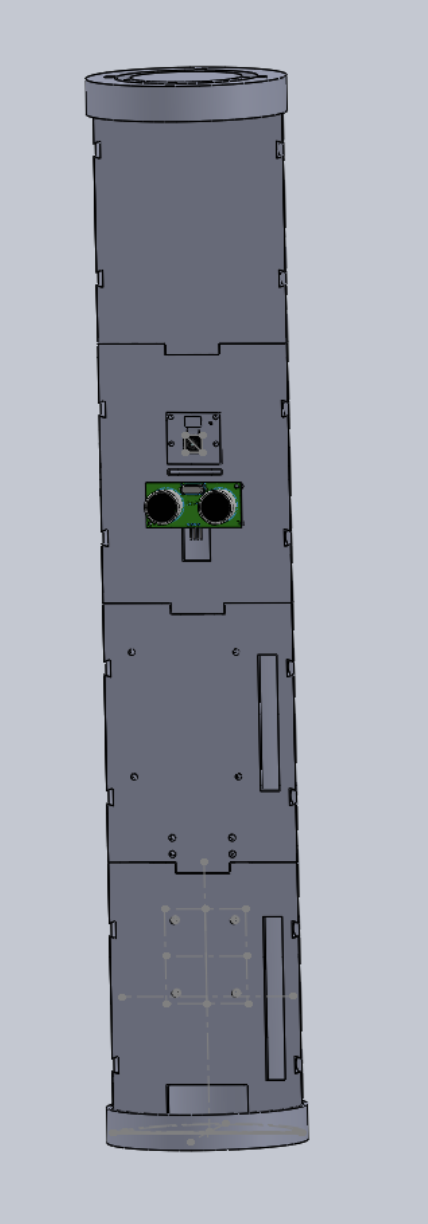
\includegraphics[width=.55\linewidth, height=8cm]{pictures/3Dprinted.png}
  \caption{CAD of The Sensor Unit: 3D printed parts assembled}
  \label{fig:CAD3dprinted}
\end{subfigure}%
\hfill
\begin{subfigure}{.4\textwidth}
  \centering
  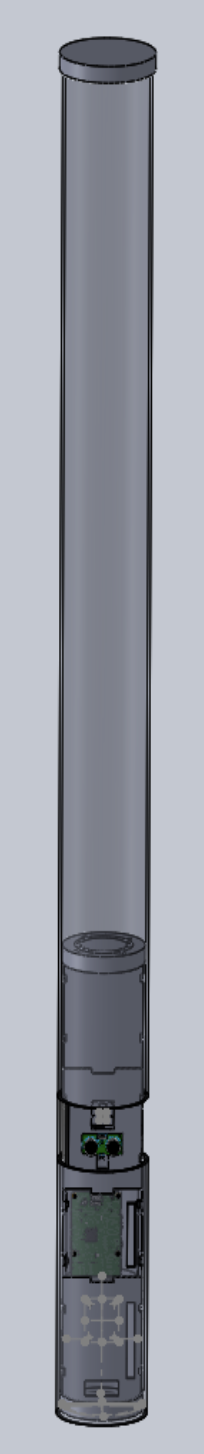
\includegraphics[width=.2\linewidth, height=8cm]{pictures/SensorTube.png}
  \caption{CAD of Sensor unit housed in a cylindrical acrylic tube}
  \label{fig:CADacrylictube}
\end{subfigure}
\caption{Our final mechanical design}
\label{fig:finalcad}
\end{figure} 
Our mechanical design prototype is comprised of 3D printed parts and an acrylic tube. 
We were limited by the factors that we wanted to create a low cost sensor housing prototype, that could be installed without having to alter a parking lot. 
Mostly due to the fact that if a parking lot has to be modified, it puts a parking lot out of commission for a period of time for construction and it is also costly to upgrade a parking lot or structure. 
It's also important to note that the mechanical design is not a major focus of our project, we just needed a method to gather data to send to the cloud. 

    We 3D printed parts most of the sensor housing system, which can all be found in our Github.\footnote{https://github.com/dfarley1/SPOT/tree/master/CAD}
There are 4 rectangular pieces that all tab and slot together. 
They can easily be glued together with tacky glue or epoxy. 
You need to put the pieces in the correct order, just so you can assembly it properly. 
We recommend taking all components to ACE hardware to get the correct sizing for each senor you would like to mount.
There are also magnets on the sides to allow for complete closure of of the 3D printed parts.
%%%%%%%%%%%%%%%%%%%%%
From top to bottom: this just a space holder, then the next panel holds both the ping and camera, following that the Raspberry  Pi is mounted, with another final bottom space holder.
% The order goes, the top piece is the top spacer then the piece that holds the sensors, then the piece that holds the raspberry pi and then then bottom spacer. 
The small lids (3.5 inches) go on either end and then you place the sensor box into the tube. 
To prepare the tube, you must cut it to the desired height and cut a window that is approximately 3 inches wide. 
This window must match up with the height of the of the 3D printed portions (once glued together).
You must also line the tube with wax paper in order to better capture the light from the pixel ring. 
This step allows for a better status indicator. 
Once assembled together it give us a sleek design of a semi circle that now fits into the acrylic tube.
Now place the 4 inch lids on either end of the tubes to help support the structure and provide a flat base. 
To hold the whole device, we obtained a 4 inch sprinkler head and the acrylic tube slides perfectly inside (after some sanding).

    For our final design, we opted for a cylindrical look to incorporate a sleek design.
Because the sensor housing device, is less than 2 feet tall, is quite short, most users would run it over easily. 
The addition of the acrylic tube was added so that users would be able to see the status of the SPOT from the car and prevent the user from running it over. 
With this iteration it was important to maximize the space of the 3D printer so each piece is approximately 4.5 to 5 inches tall each. 
Combined all together with some glue, the 3D printed portion of the mechanical design holds the camera and ping sensor at a proper height of 10-11 inches off the ground.
This is so that our prototype can detect whether or not a car is right in front of it or not. 
The Raspberry Pi is hidden inside the semi circle so that all the wires are enclosed and it is neat and tidy from an outside point of view. 
We also added some magnets to help enclose the entire module. 
This way we can open and close the module with ease whenever we need to do some testing. 
The 3D printed parts were very sturdy, however it took a long time to print one set in order to assemble the whole system.

\begin{figure}
\centering
\begin{subfigure}{.4\textwidth}
  \centering
  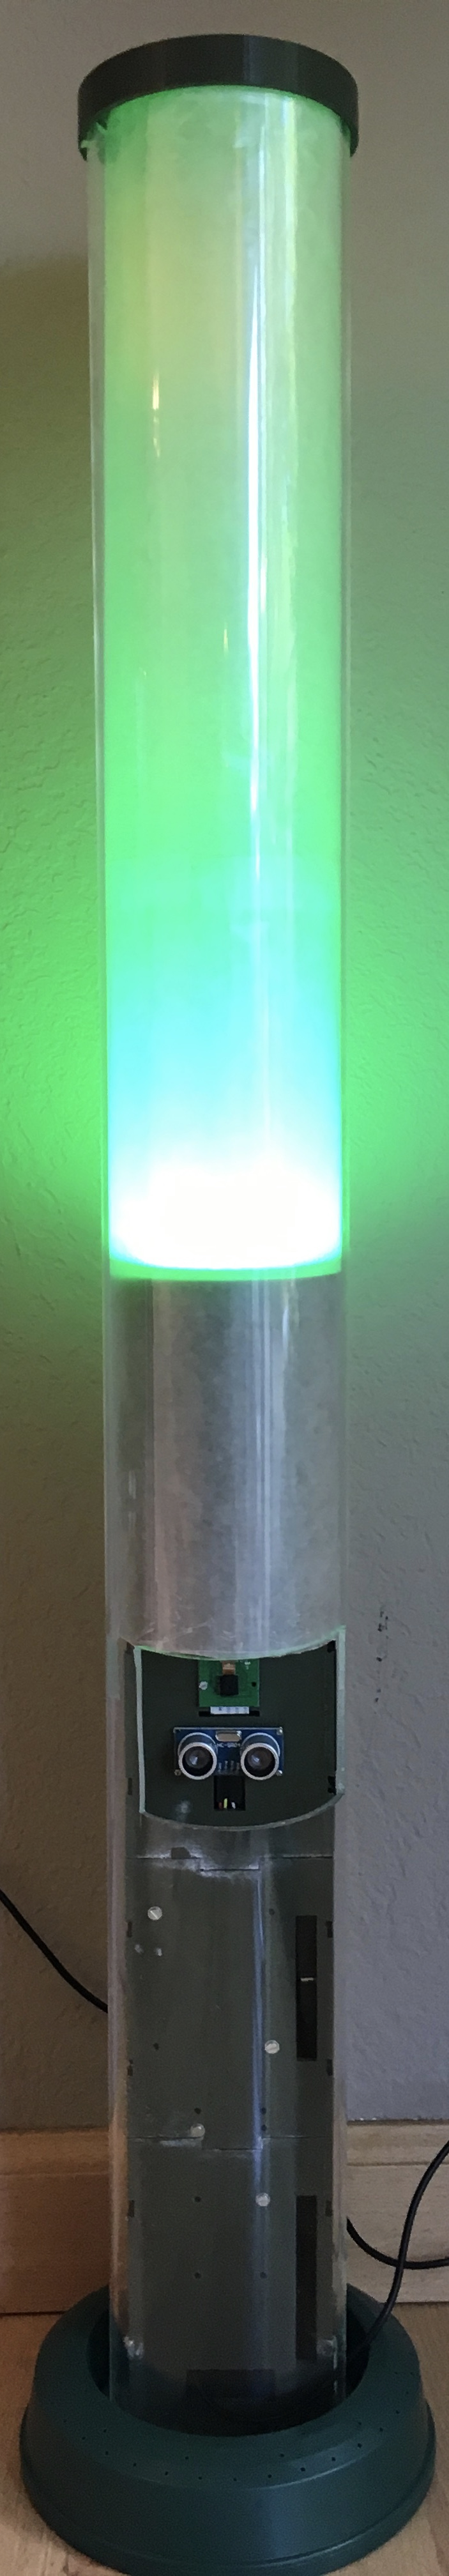
\includegraphics[width=.25\linewidth,height=9cm]{pictures/fullsizeoutput_14d.jpeg}
  \caption{Physical Prototype: SPOT with status: Occupied}
  \label{fig:3dprintedassembly}
\end{subfigure}%
\hfill
\begin{subfigure}{.4\textwidth}
  \centering
  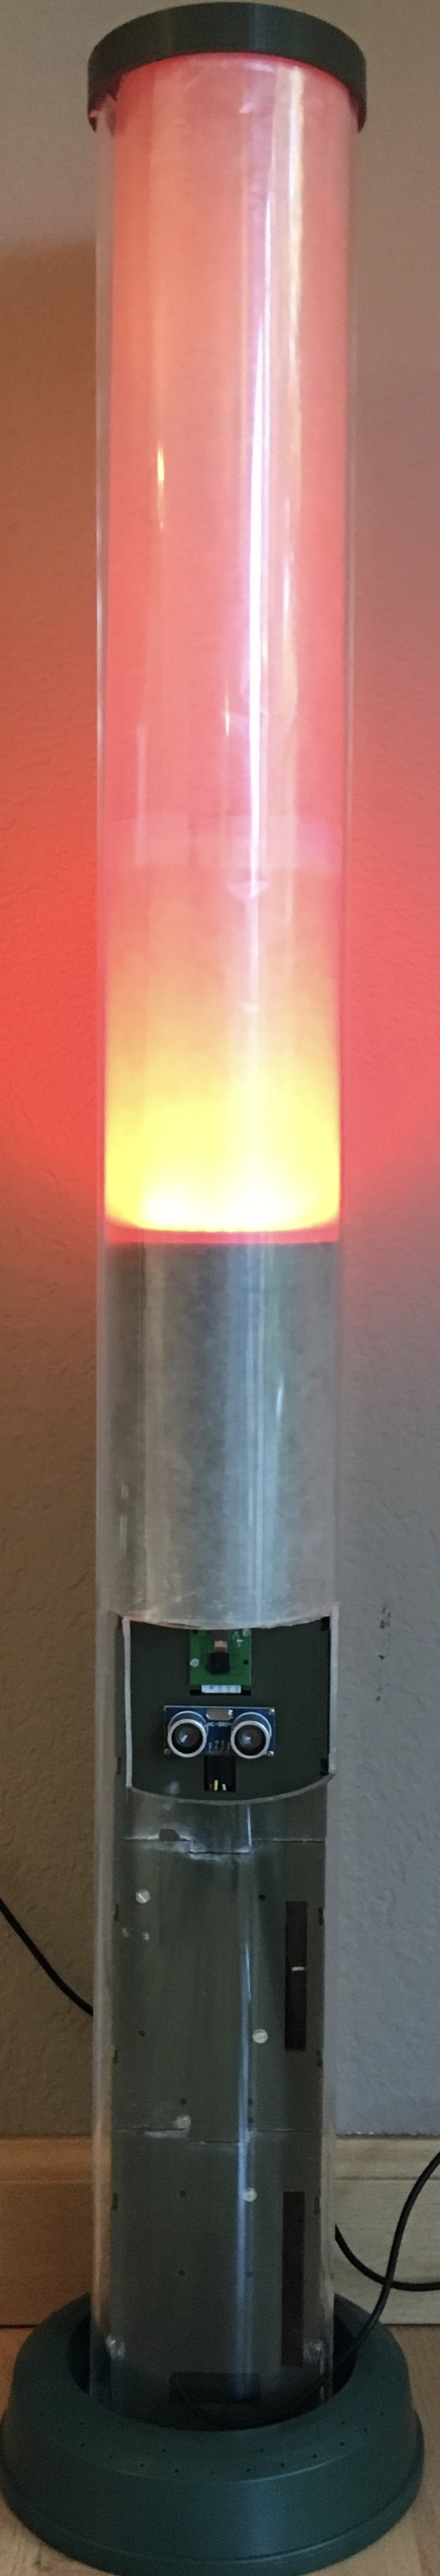
\includegraphics[width=.25\linewidth,height=9cm]{pictures/fullsizeoutput_14f.jpeg}
  \caption{Physical Prototype: SPOT with status: Unoccupied}
  \label{fig:acrylictubefullassembly}
\end{subfigure}
\caption{Physical Prototype: Side By Side of Status Lights with Acrylic Tube}
\label{fig:finalassembly}
\end{figure}
